\documentclass[12pt,mathserif]{beamer}
\usepackage[no-math]{fontspec}%
\usepackage{xunicode,xltxtra,beamerthemesplit}
\usepackage{amsmath,mathrsfs,amscd,graphicx}
\usepackage{algorithm2e}
\usetheme{CambridgeUS}

\setsansfont{Kai} 

\XeTeXlinebreaklocale "zh"
\XeTeXlinebreakskip=0pt plus 1pt minus 0.1pt


\begin{document}
\title{\XeTeX 新手入门}
\author{作者}
\institute[电子邮件]{我的单位}
\frame{\titlepage}

\frame{\frametitle{这是中文测试}
慈母手中线,\\
游子身上衣。\\
临行密密缝,\\
意恐迟迟归。\\
谁言寸草心,\\
报得三春晖?\\
}

\frame{\frametitle{This English Test}
This is English test!
\begin{equation}
\alpha +\beta=\gamma
\end{equation}
\begin{equation}
x^2+y^2=z^{\sin x}
\end{equation}
}

\frame{\frametitle{Algorithm layout}
\begin{algorithm}[H]
\caption{\textsc{Path-Count}$(G, P, s, t)$}
\If{$s = t$}{
  \Return $1$\\
}\Else{
  $S \leftarrow 0$\\
  \ForEach{parent vertex $w$ of $t$}{
    \If{$P[w]$ = nil} {
      $P[w]\leftarrow $\textsc{Path-Count}$(G, P, s, w)$
    }
    $S\leftarrow S + P(w)$
  }
  \Return $S$
}
\end{algorithm}
}

\frame{\frametitle{Insert picture}
\begin{center}
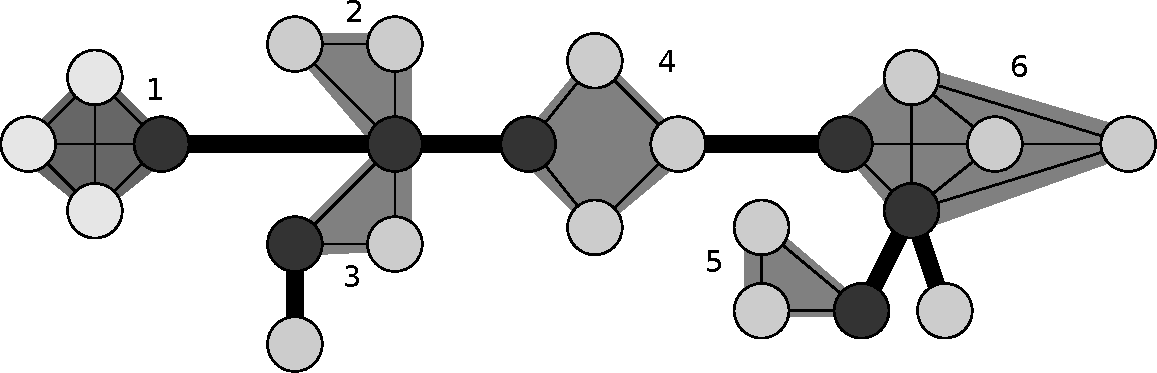
\includegraphics[width=300pt]{hw5-fig-22-10.pdf}
\end{center}
}

\end{document}

